\documentclass[11pt]{beamer}
\usepackage{helvet} %font
\beamertemplatenavigationsymbolsempty
\usetheme{JuanLesPins}
\usefonttheme{structurebold}

\usepackage[french]{babel}
\usepackage[utf8]{inputenc}
\usepackage[T1]{fontenc}
\usepackage{amssymb,amsmath}
\usepackage{tikz}
\usepackage{geometry}
\usepackage{xcolor,colortbl}
\usetikzlibrary{arrows,positioning}
\usepackage{listings}

\AtBeginSubsection[]
{
   \begin{frame}
	\small \tableofcontents[currentsection]
   \end{frame}
}

\newenvironment{slide}[1]{%
\begin{frame}[environment=slide]
\frametitle{#1}
}{%
\end{frame}
}
\setbeamercolor{structure}{fg=red}
\setbeamercolor{frametitle}{bg=black,fg=white}
\definecolor{gris}{gray}{0.6}
\definecolor{grisclair}{gray}{0.9}

\newtheorem{exercice}{Exercice}

\title{Machine Learning IV \\ Classification non supervisée}
\author{Nicolas Bourgeois}
\date{}

\newcommand{\Python}[1]{
	{\small	\lstinputlisting[language=Python]{./#1.py}}
}
\newenvironment{pyenvsmall}
	{ \ttfamily \tiny }
	{\par  }

\newcommand{\Pythonsmall}[1]{
	{\scriptsize \lstinputlisting[language=Python]{./#1.py}}
}
\newcommand{\elimine}[1]{{\textcolor{lightgray}{#1}}}

\newcommand\Wider[2][3em]{%
\makebox[\linewidth][c]{%
  \begin{minipage}{\dimexpr\textwidth+#1\relax}
  \raggedright#2
  \end{minipage}%
  }%
}

\begin{document}

\begin{frame}
\maketitle
\end{frame}

\begin{frame}{K-means : objectif}

On dispose de n données et de p variables.\\

\pause
\vspace{0.2cm}

On veut créer une partition qui minimise la somme des inerties internes à chaque classe.\\

$$\min \sum_{i \leq k} \sum_{x \in Z_i} d^2(x,\bar{z}_i)$$
où $\bar{z_i}$ est le centre de $Z_i$.

\end{frame}

\begin{frame}{K-means : base}

On initialise les centres aléatoirement, puis à chaque étape :
\pause
\begin{itemize}
	\item On affecte chaque donnée au centre le plus proche
	\item On recalcule la position des centres
\end{itemize}

\end{frame}


\begin{frame}{Exercice}

\begin{exercice}
Importez les données iris avec \texttt{dataset.load\_iris}. Effectuez un k-means avec 2,3,4 valeurs. Comparez graphiquement les résultats avec les valeurs cibles.
\end{exercice}

Attention : L'objectif ici n'est pas de prédire Y, mais de mettre en correspondance Y avec un clustering ne dépendant que de X.

\end{frame}

\begin{frame}{Résultat attendu}
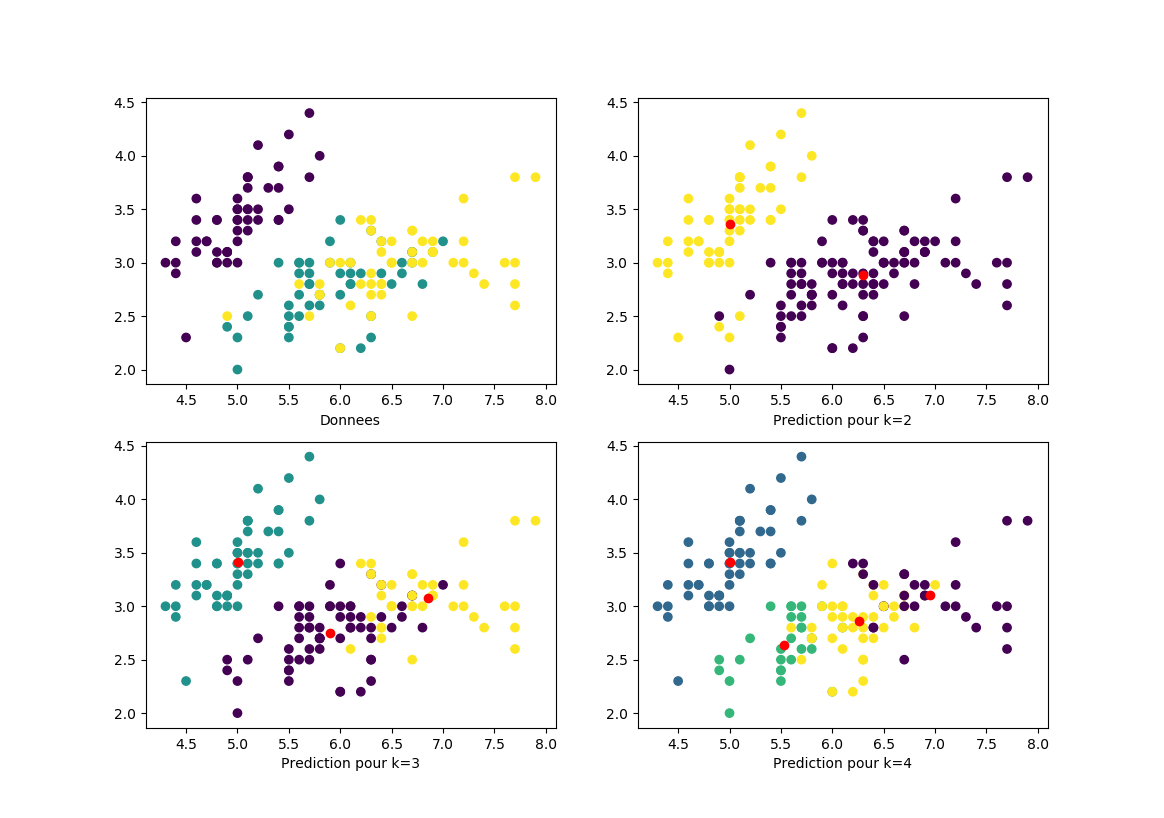
\includegraphics[scale=0.35]{ex501}
\end{frame}

\begin{frame}{Solution}
\Pythonsmall{ex501}
\end{frame}


\begin{frame}{Exercice}

\begin{exercice}
Séparez maintenant vos données en un échantillon d'apprentissage et un échantillon de test. Visualisez (par exemple avec des différences d'opacité) dans quels clusters sont placées les nouvelles valeurs.
\end{exercice}

\end{frame}

\begin{frame}{Résultat attendu}
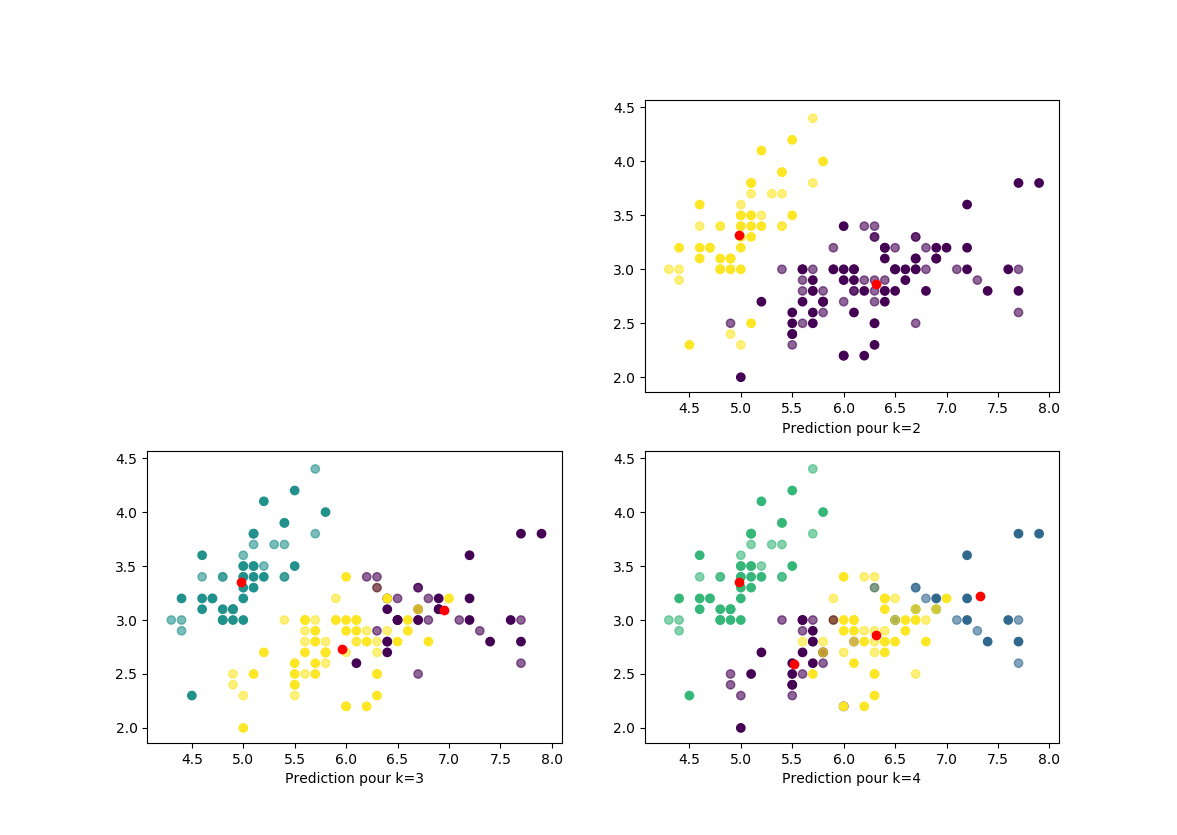
\includegraphics[scale=0.35]{ex501bis}
\end{frame}

\begin{frame}{Solution}
\Pythonsmall{ex501bis}
\end{frame}


\begin{frame}{Problèmes}

\begin{itemize}
	\item Pas de garantie d'optimalité
	\item Pas de garantie de polynomialité (par rapport à n)
	\item Choisir k a priori
\end{itemize}

\end{frame}

%%%%%%%%%%%%%%%%%%%%%%%%%%%%%%%%%%%%


\begin{frame}{CHA : objectif}

On dispose de n données et de p variables, qu'on veut regrouper en un nombre a priori inconnu de clusters.\\

\end{frame}

\begin{frame}{K-means : base}

Initialement, tous les points sont séparés chacun dans un cluster. A chaque étape :
\pause
\begin{itemize}
	\item On calcule la paire de clusters de moindre dissimilarité,
	\item On fusionne les clusters en question,
	\item On met à jour les mesures de dissimilarité avec les autres clusters
\end{itemize}

\end{frame}

\begin{slide}{Exemple}

\begin{tikzpicture}

\node[shape=rectangle,fill=red] (1) at (0,0){};
\node[shape=rectangle,fill=red] (2) at (0,1){};
\node[shape=rectangle,fill=red] (3) at (1,2){};
\node[shape=rectangle,fill=red] (4) at (2,1){};
\node[shape=rectangle,fill=red] (5) at (4,2){};
\node[shape=rectangle,fill=red] (6) at (5,3){};
\node[shape=rectangle,fill=red] (7) at (6,2.5){};
\node[shape=rectangle,fill=red] (8) at (7,1){};
\node[shape=rectangle,fill=red] (9) at (5.5,1.5){};
\pause
\draw[dashed] (-0.3,-0.3) rectangle (0.3,1.3);
\pause
\draw[dashed] (4.7,2.2) rectangle (6.3,3.3);

\end{tikzpicture}

\end{slide}

\begin{slide}{Exemple}

\begin{tikzpicture}

\node[shape=rectangle,fill=red] (1) at (0,0){};
\node[shape=rectangle,fill=red] (2) at (0,1){};
\node[shape=rectangle,fill=red] (3) at (1,2){};
\node[shape=rectangle,fill=red] (4) at (2,1){};
\node[shape=rectangle,fill=red] (5) at (4,2){};
\node[shape=rectangle,fill=red] (6) at (5,3){};
\node[shape=rectangle,fill=red] (7) at (6,2.5){};
\node[shape=rectangle,fill=red] (8) at (7,1){};
\node[shape=rectangle,fill=red] (9) at (5.5,1.5){};
\draw[dashed] (-0.3,-0.3) rectangle (0.3,1.3);
\draw[dashed] (4.7,1.2) rectangle (6.3,3.3);
\pause
\draw[dashed] (0.7,0.7) rectangle (2.3,2.3);

\end{tikzpicture}

\end{slide}

\begin{slide}{Exemple}

\begin{tikzpicture}

\node[shape=rectangle,fill=red] (1) at (0,0){};
\node[shape=rectangle,fill=red] (2) at (0,1){};
\node[shape=rectangle,fill=red] (3) at (1,2){};
\node[shape=rectangle,fill=red] (4) at (2,1){};
\node[shape=rectangle,fill=red] (5) at (4,2){};
\node[shape=rectangle,fill=red] (6) at (5,3){};
\node[shape=rectangle,fill=red] (7) at (6,2.5){};
\node[shape=rectangle,fill=red] (8) at (7,1){};
\node[shape=rectangle,fill=red] (9) at (5.5,1.5){};
\draw[dashed] (-0.3,-0.3) rectangle (0.3,1.3);
\draw[dashed] (3.7,1.2) rectangle (6.3,3.3);
\draw[dashed] (0.7,0.7) rectangle (2.3,2.3);

\end{tikzpicture}

\end{slide}


\begin{frame}{Exercice}
\begin{exercice}
Importez les données iris. Effectuez une classification hiérarchique ascendante avec la distance de Ward. Fixez un seuil optimal ou un nombre de compsantes. Représentez graphiquement les clusters et comparez avec les valeurs de Y.
\end{exercice}
\end{frame}

\begin{frame}{Résultat attendu}
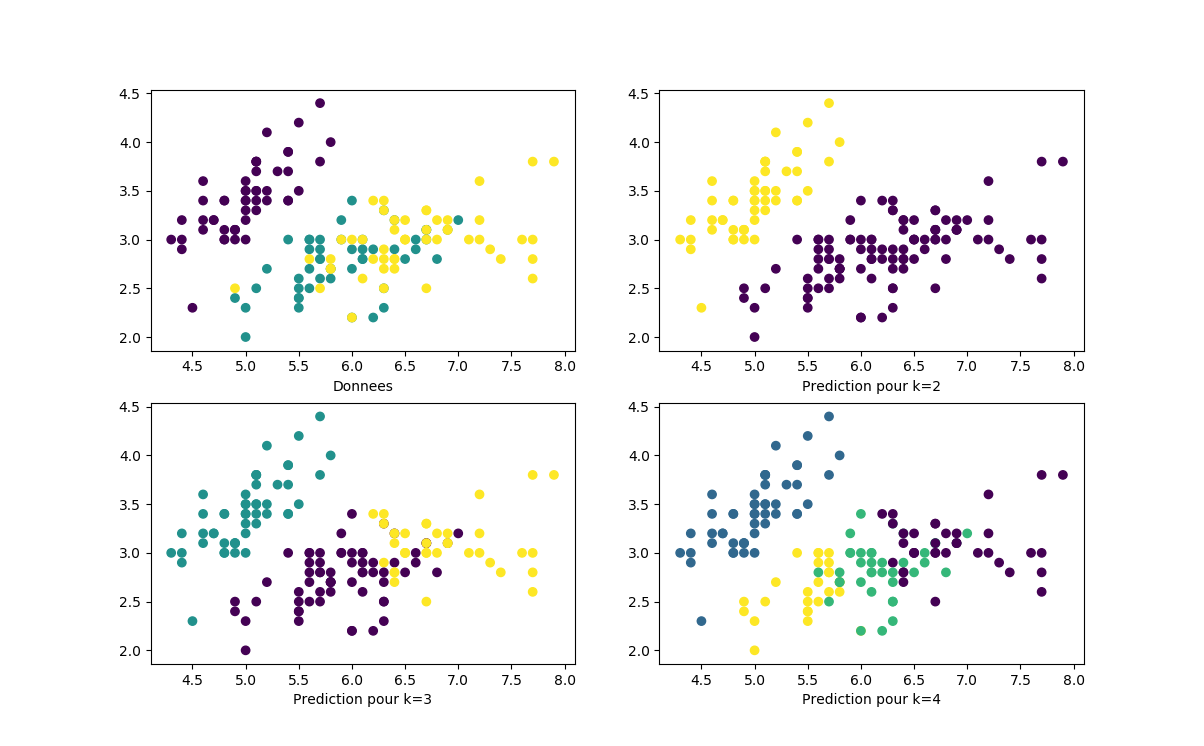
\includegraphics[scale=0.35]{ex504}
\end{frame}

\begin{frame}{Solution}
\Pythonsmall{ex504}
\end{frame}

\begin{frame}{Exercice}
\begin{exercice}
Importez les données du titanic et ne conservez que les champs \textit{age} et \textit{fare}. Représentez côte à côte les résultats d'une classification hiérarchique et d'un kmeans à quatre et cinq clusters.
\end{exercice}
\begin{exercice}
Même chose, mais commencez par normaliser les données avec MinMaxScaler.
\end{exercice}
\end{frame}

\begin{frame}{Résultat attendu (1)}
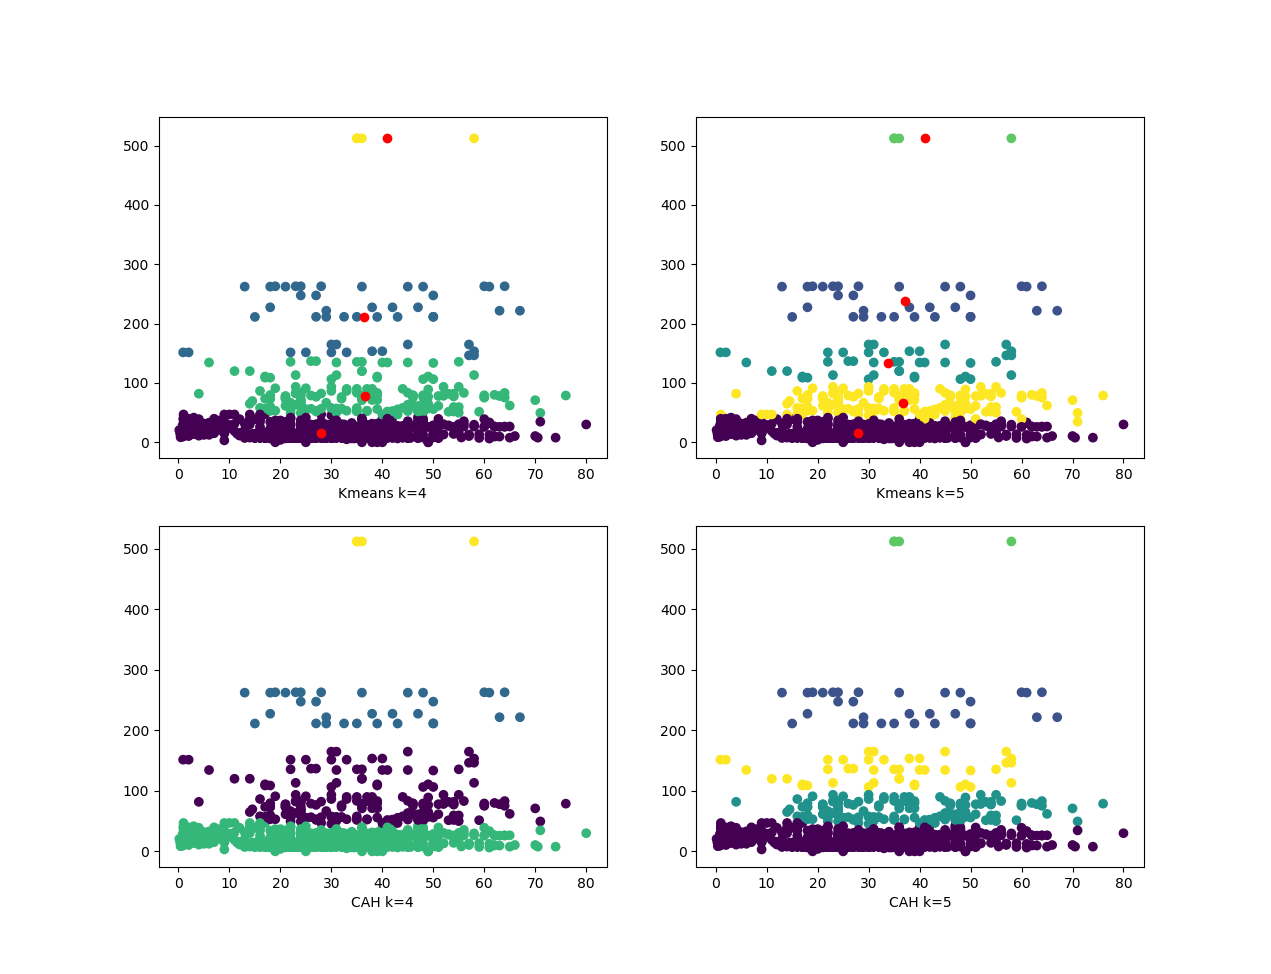
\includegraphics[scale=0.3]{ex505}
\end{frame}

\begin{frame}{Solution (1)}
\Pythonsmall{ex505}
\end{frame}


\begin{frame}{Résultat attendu (2)}
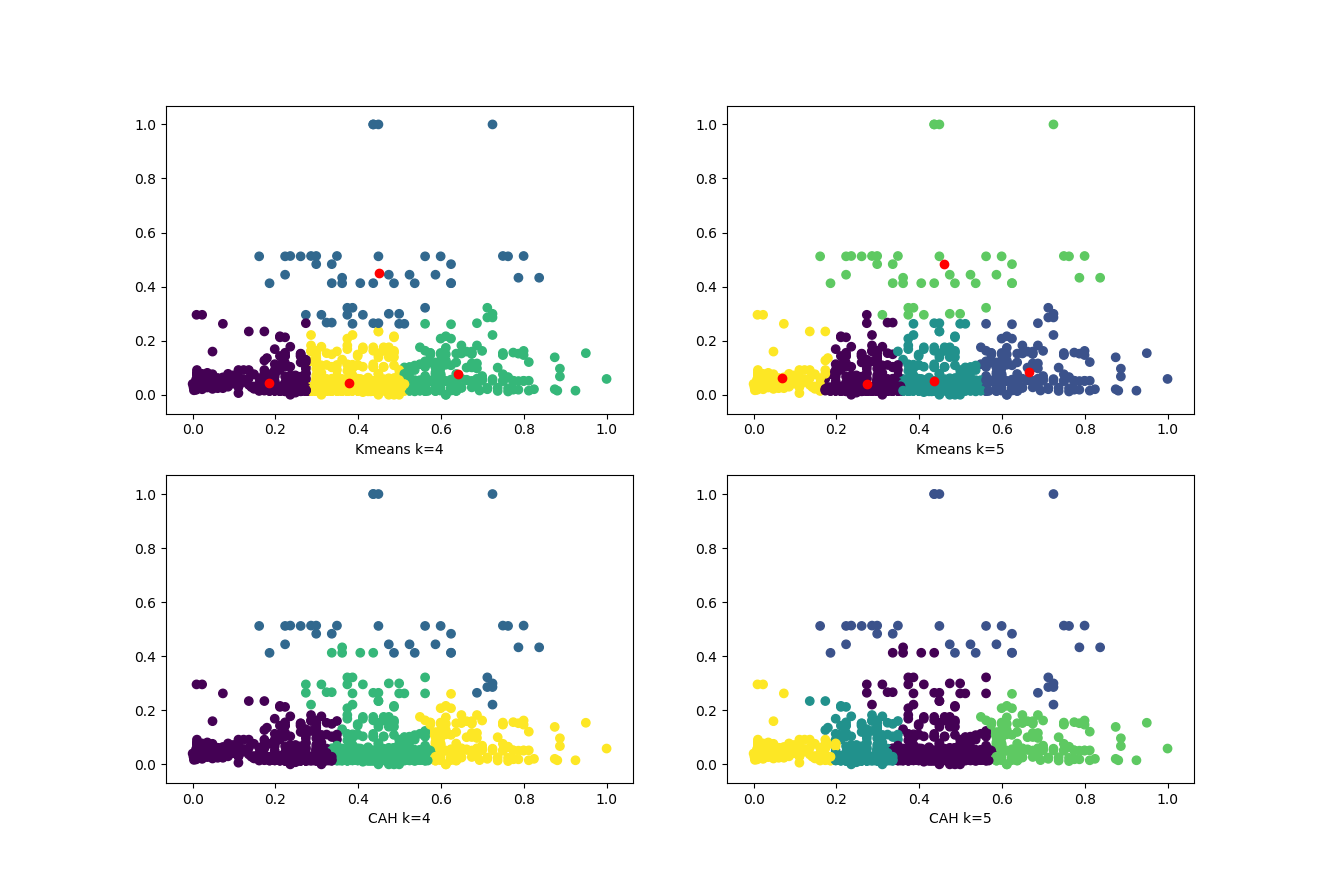
\includegraphics[scale=0.3]{ex506}
\end{frame}

\begin{frame}{Solution (2)}
\Pythonsmall{ex506}
\end{frame}

\begin{frame}{Comparaison de méthodes}
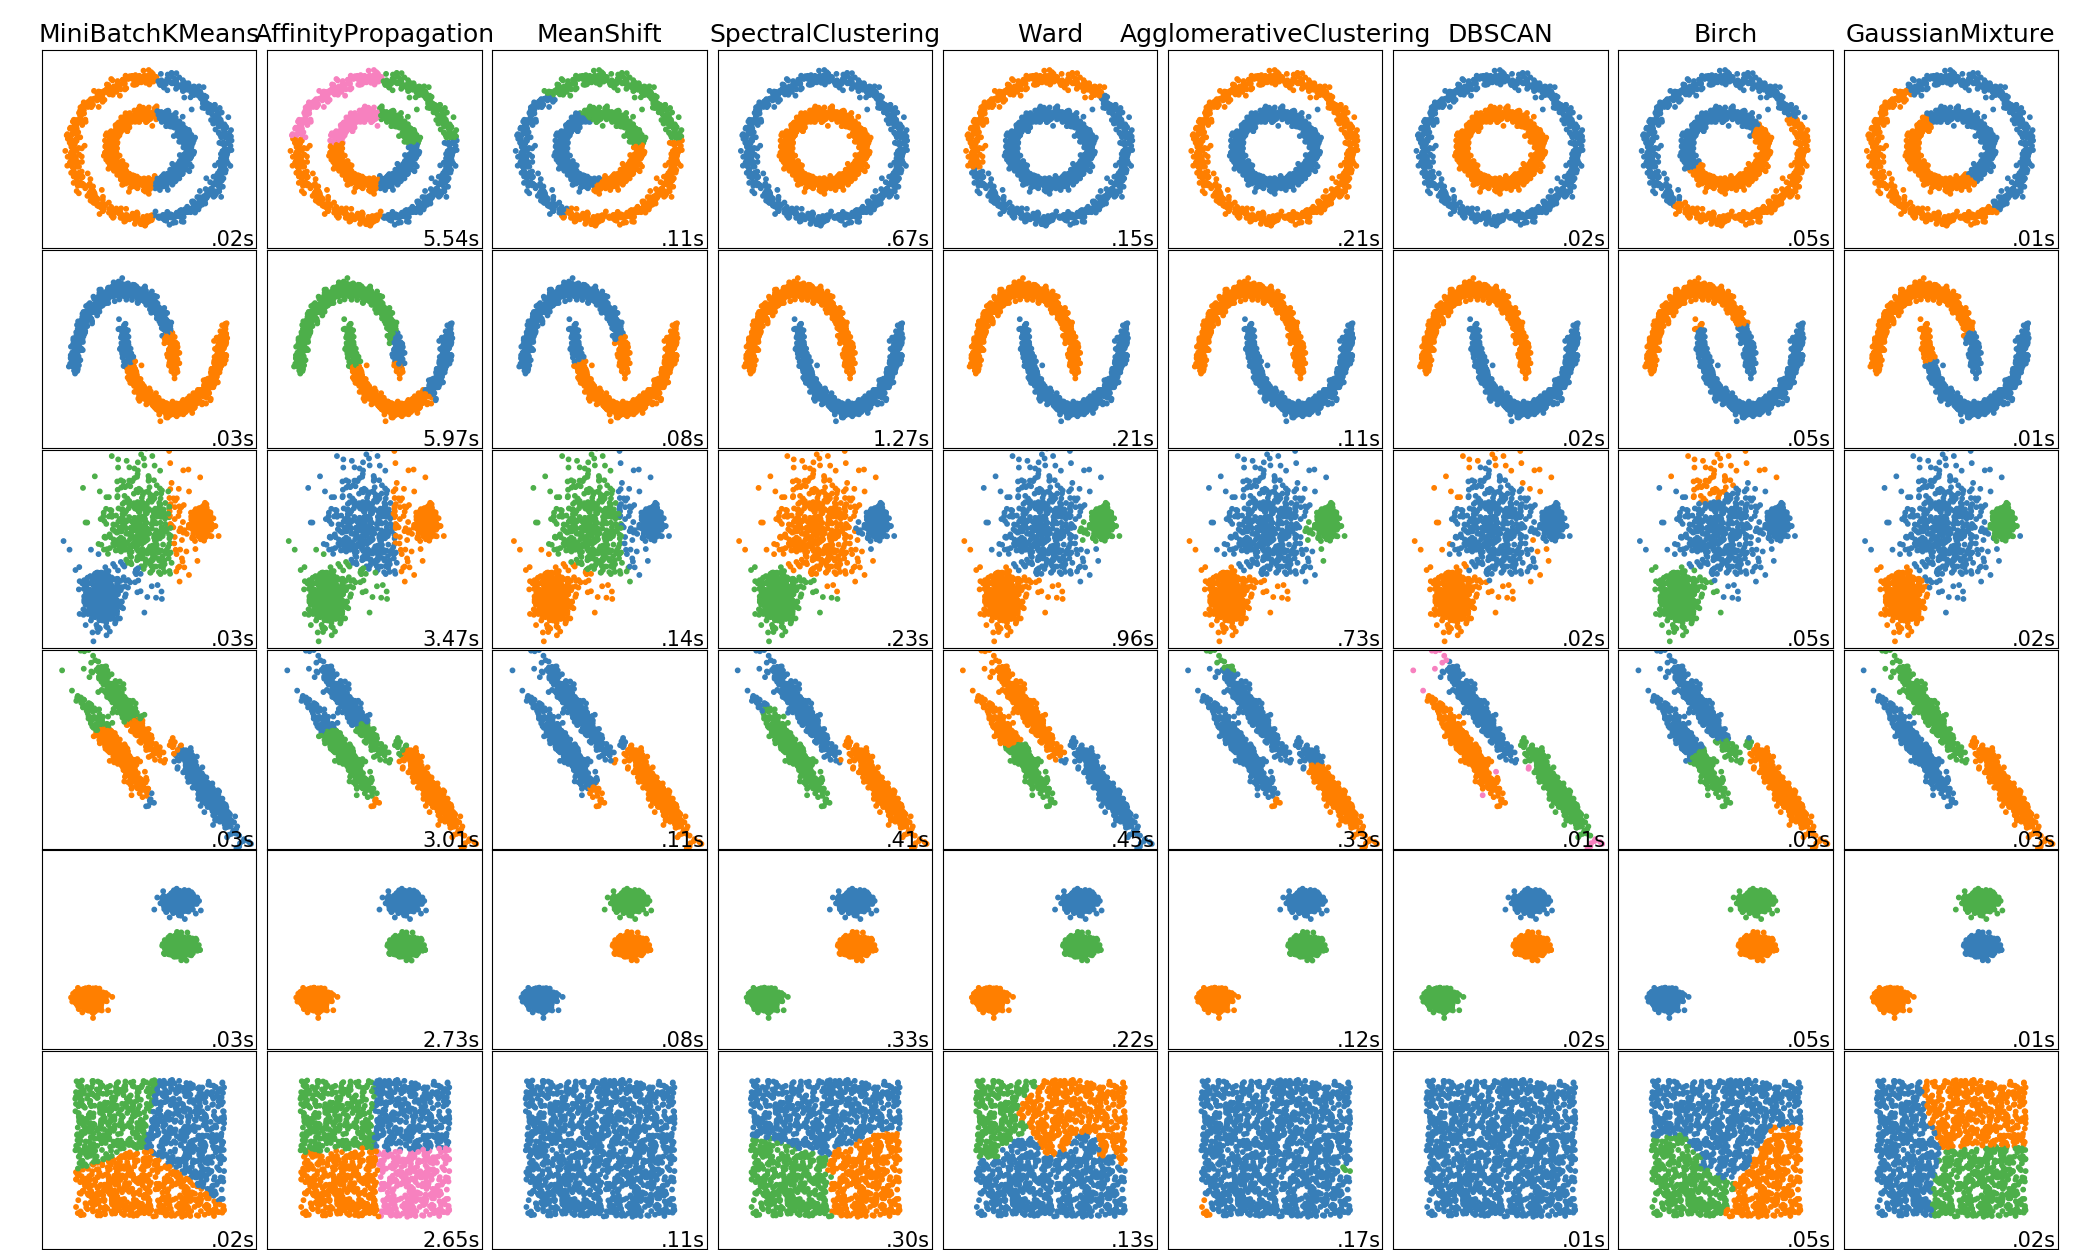
\includegraphics[scale=0.2]{cluster_comparison}
\end{frame}

\end{document}

